%! TEX program = lualatex

%Government regulation Google Slide Doc: https://docs.google.com/presentation/d/1hYz59aNMrl8NCRxDNwFzt7CL7TeKdDwXjqiq0pOHfrE/edit?usp=sharing

\documentclass[nobackground,dvipsnames,table]{beamer}
%\usepackage{sio}
\usepackage{tsc}
\usepackage{pdfpc}
\usepackage{pgfpages}
\usepackage{multimedia}

%%%%%%%% edit hyperlink colors %%%%%%%%
\hypersetup{
  colorlinks   = true, 
  urlcolor     = tscurl, % color of external hyperlinks
  linkcolor    = white,   % color of internal links
}

%%%%% the below command allows custom highlights used in this presentation with \hlc %%%%%%
\makeatletter
\let\HL\hl
\renewcommand\hl{%
  \let\set@color\beamerorig@set@color
  \let\reset@color\beamerorig@reset@color
  \HL}
\makeatother

\newcommand{\hlc}[2][yellow]{{%
    \colorlet{foo}{#1}%
    \sethlcolor{foo}\hl{#2}}%
}   
%%%%%%%%%%%%%%%%%%%%%%%%%%%%%%%%%%%%%%%%%%%

\mode<presentation>
{\usetheme{default}
	\usecolortheme{tsc}
	\setbeamercovered{transparent}
	\useinnertheme[shadow=false]{rounded}
	\usebackgroundtemplate{}
	\setbeamercolor*{frametitle}{parent=palette primary}
	\setbeamerfont{block title}{size={}}
	\setbeamertemplate{navigation symbols}{}
    \setbeamertemplate{itemize items}[circle]
        \setbeamertemplate{enumerate items}[circle]

}
%{\usetheme{Hannover}
%	\usecolortheme{sio}
%	\setbeamercovered{transparent}
%	\useinnertheme[shadow=false]{rounded}
%	\usebackgroundtemplate{}
%	\setbeamercolor*{frametitle}{parent=palette primary}
%	\setbeamerfont{block title}{size={}}
%	\setbeamertemplate{navigation symbols}{}
%}

%%%%%%%%%%%%%%%%%%%%%%%%%%%%%%%%%%
%%%% slide 1 on google slides %%%%
%%%%%%%%%%%%%%%%%%%%%%%%%%%%%%%%%%
\title[Governments \& the Internet]{\LARGE{Governments \& the Internet}}
\subtitle{\small{\emph{The laws that shape speech online}}}

\author[Maxim]{\large{Karen Maxim}}
%\institute[SIO]{\large Stanford Internet Observatory}
\date[]{} 
\subject{Trust and Safety}
\AddToShipoutPictureBG*{
  \AtPageLowerLeft{\hspace{-0.4cm}
    
\includegraphics[width=13.1cm]{img/consortium-image}}
}


% Change this to make a file with just slides, just notes or both
%\setbeameroption{hide notes}                 % Only slides
%\setbeameroption{show only notes}            % Only notes
\setbeameroption{show notes on second screen} % Both

\begin{document}

%\coverpage

\begin{frame}
	\titlepage
\end{frame}


\section{Introduction}

%%%%%%%%%%%%%%%%%%%%%%%%%%%%%%%%%%
%%%% slide 2 on google slides %%%%
%%%%%%%%%%%%%%%%%%%%%%%%%%%%%%%%%%
\begin{frame}{Learning objectives}
	Today we will:
	\begin{itemize}
		\item Learn about the laws that govern speech on the Internet
		\item And how tech companies make decisions about them
	\end{itemize}
\end{frame}


%%%%%%%%%%%%%%%%%%%%%%%%%%%%%%%%%%
%%%% slide 3 on google slides %%%%
%%%%%%%%%%%%%%%%%%%%%%%%%%%%%%%%%%
\begin{frame}{Why Silicon Valley and not Silizium Schlucht?}
\footnotesize{
American laws and the American legal system created the conditions necessary for the Internet to come into existence, at least the Internet as it looks \emph{right now}. 
\vspace{0.5ex}

U.S. law is special in some important areas:
\begin{itemize}
    \item \textbf{Intermediary liability} - whether Internet companies (aka “intermediaries” between speakers and hearers) are responsible for the speech their users post
    \item \textbf{Intellectual property} - how companies protect their IP and whether they’re responsible for their users’ IP violations
    \item \textbf{Privacy} - What are companies’ obligations to protect user privacy/personal information?
    \item \textbf{Corporate} - How companies form, take on investment, operate, and owners’ liability if things go wrong
    \item \textbf{The First Amendment} - limits the ability of US government actors to act against speech they dislike. 1A is a deeply embedded cultural norm - both what it does, and what we \emph{think} it does 
\end{itemize}

We’re going to focus on \textbf{Intermediary Liability} and a bit on \textbf{First Amendment}.
}

\note[]{Bonus reading:
Anupam Chander, How Law Made Silicon Valley, 63 Emory L. J. 639 (2014).}
        
\end{frame}


\section{Overall U.S. Approach to Internet policy}
%%%%%%%%%%%%%%%%%%%%%%%%%%%%%%%%%%
%%%% slide 4 on google slides %%%%
%%%%%%%%%%%%%%%%%%%%%%%%%%%%%%%%%%
\begin{frame}{Overall U.S. Approach to Internet policy}
	The U.S. has taken a deliberately laissez-faire approach to Internet regulation. \newline
        \newline Here are the first three principles of the Clinton Administration’s 1997 \href{https://clintonwhitehouse4.archives.gov/WH/New/Commerce/read.html}{“Framework for Global Electronic Commerce”}: 
        \begin{enumerate}
            \item The private sector should lead.
            \item  Governments should avoid undue restrictions on electronic commerce.
            \item Where governmental involvement is needed, its aim should be to support and enforce a predictable, minimalist, consistent and simple legal environment for commerce.
        \end{enumerate}
        \note[]{https://clintonwhitehouse4.archives.gov/WH/New/Commerce/read.html}
\end{frame}

\begin{frame}{Overall U.S. Approach to Internet policy}
	Now we have 30 years of court decisions, legislative* and regulatory** action and inaction, mostly consistent with the Framework. \newline \newline The Framework remains a good summary of U.S. tech policy, though there’s growing appetite to regulate tech more.\newline\newline

    \footnotesize{* This means lawmakers like Congress and state legislatures}
    \newline
    \footnotesize{** This means agencies like the Federal Trade Commission or the Federal Communications Commission.}
\end{frame}



\section{Intermediary Liability and Section 230}

%%%%%%%%%%%%%%%%%%%%%%%%%%%%%%%%%%
%%%% slide 5 on google slides %%%%
%%%%%%%%%%%%%%%%%%%%%%%%%%%%%%%%%%
\begin{frame}{Intermediary liability \newline \small{“The 26 Words That Created The Internet”*}}

\footnotesize{
Here is "Section 230" (the exact legal citation is 47 U.S. Code Section 230(c)):
}
        
\scriptsize{ 
    \begin{itemize}
        \item [\footnotesize{\textbf{(c)}}] \textbf{Protection for “Good Samaritan” blocking and screening of offensive material}
        
        \begin{itemize}
            \scriptsize{
            \item[(1)] \underline{Treatment of publisher or speaker}
            }
        \end{itemize}
        
        \item[] No provider or user of an interactive computer service shall be treated as the publisher or speaker of any information provided by another information content provider.
    \end{itemize}

    \begin{itemize}
        \item []
        \begin{itemize}
            \scriptsize{
            \item [(2)] \underline{Civil liability}
            }
        \end{itemize}
        
        \item[] No provider or user of an interactive computer service shall be held liable on account of—

        \begin{itemize}
            \scriptsize{
            \item[(A)] any action voluntarily taken in good faith to restrict access to or availability of material that the provider or user considers to be obscene, lewd, lascivious, filthy, excessively violent, harassing, or otherwise objectionable, whether or not such material is constitutionally protected; or
            \item[(B)] any action taken to enable or make available to information content providers or others the technical means to restrict access to material described in paragraph (1)
            }
        \end{itemize}
    \end{itemize}
    }

    \tiny{\emph{*and the title of a great book by Jeff Kosseff, a professor at the U.S. Naval Academy}}

    \note[]{Read this aloud together with the students in its entirety as you would a sacred text. Or divvy up the sections and have different students read them aloud.}
\end{frame}

%%%%%%%%%%%%%%%%%%%%%%%%%%%%%%%%%%
%%%% slide 6 on google slides %%%%
%%%%%%%%%%%%%%%%%%%%%%%%%%%%%%%%%%
\begin{frame}{How does Section 230 work?} 
        
\scriptsize{ 
    \begin{itemize}
        \item [\footnotesize{\textbf{(c)}}] \textbf{Protection for “Good Samaritan” blocking and screening of offensive material}
        
        \begin{itemize}
            \scriptsize{
            \item[(1)] \underline{Treatment of publisher or speaker}
            }
        \end{itemize}
        
        \item[] \hlc[blue!20]{No provider or user of an }\hlc[red!60]{interactive computer}\hlc[blue!20]{ service shall be treated as the publisher or speaker of any information provided by }\hlc[violet!30]{another information content provider.}
    \end{itemize}

    \begin{itemize}
        \item []
        \begin{itemize}
            \scriptsize{
            \item [(2)] \underline{\hlc[red!40]{Civil liability}}
            }
        \end{itemize}
        
        \item[] No provider or user of an interactive computer service shall be held liable on account of—

        \begin{itemize}
            \scriptsize{
            \item[(A)] \hlc[teal!40]{any action voluntarily taken} in good faith to restrict access to or availability of material that the provider or user considers to be obscene, lewd, lascivious, filthy, excessively violent, harassing, or \hlc[orange!60]{otherwise objectionable}, whether or not such material is constitutionally protected; or
            \item[(B)] any action taken to enable or make available to information content providers or others the technical means to restrict access to material described in paragraph (1)
            }
        \end{itemize}
    \end{itemize}
    }
\note[]{
\scriptsize{
\hlc[blue!20]{Blue highlight}: This is an extraordinary sentence, because of its simplicity and its scope. All over U.S. law, there are instances in which someone can be held liable for the actions of another. This happens in criminal law (i.e. accomplices), in tort law, in copyright law (companies have to take down copyright violations posted by others), in corporate law (companies are responsible for the actions of their employees). Sometimes publishers like newspapers are liable for the speech they publish, as in defamation law. Section 230, by contrast, protects internet companies from liability for almost all the speech of others. Early court cases interpreting section 230 immunized tech companies from liability even when speech they hosted caused serious harm - criminal harm! - to real people. \newline 

\textbf{[Placeholder to discuss the implications of the Gonzalez v. Google case, decision expected in summer 2023.  Do recommendation algorithms count as conduct by Google for for which it can be held liable?]} \newline 

\hlc[red!60]{Red highlight}: Interactive computer service is defined so broadly as to give basically every website, service, marketplace or app the protections of Section 230. It even covers infrastructure-type services like AWS or Cloudflare. \newline 
}}
\end{frame}

\begin{frame}{How does Section 230 work?} 
        
\scriptsize{ 
    \begin{itemize}
        \item [\footnotesize{\textbf{(c)}}] \textbf{Protection for “Good Samaritan” blocking and screening of offensive material}
        
        \begin{itemize}
            \scriptsize{
            \item[(1)] \underline{Treatment of publisher or speaker}
            }
        \end{itemize}
        
        \item[] \hlc[blue!20]{No provider or user of an }\hlc[red!60]{interactive computer}\hlc[blue!20]{ service shall be treated as the publisher or speaker of any information provided by }\hlc[violet!30]{another information content provider.}
    \end{itemize}

    \begin{itemize}
        \item []
        \begin{itemize}
            \scriptsize{
            \item [(2)] \underline{\hlc[red!40]{Civil liability}}
            }
        \end{itemize}
        
        \item[] No provider or user of an interactive computer service shall be held liable on account of—

        \begin{itemize}
            \scriptsize{
            \item[(A)] \hlc[teal!40]{any action voluntarily taken} in good faith to restrict access to or availability of material that the provider or user considers to be obscene, lewd, lascivious, filthy, excessively violent, harassing, or \hlc[orange!60]{otherwise objectionable}, whether or not such material is constitutionally protected; or
            \item[(B)] any action taken to enable or make available to information content providers or others the technical means to restrict access to material described in paragraph (1)
            }
        \end{itemize}
    \end{itemize}
    }
\note[]{

\scriptsize{\textbf{NOTE: duplicate slide created to make space for the rest of the notes.}} \newline 
\tiny{
\hlc[violet!30]{Purple highlight}: To be protected by Section 230, the content at issue has to be provided by someone else - “another” information content provider, “in whole or in part” [this comes from the definition of information content provider].  You \textbf{can} sue Twitter for content created BY Twitter, for example. There’s a court decision about a site called Roommates.com in which was held liable for a dropdown menu that invited users to violate federal and state fair housing laws. One way a plaintiff can try to survive a motion to dismiss when suing a platform about content is to argue that the platform was responsible at least “in part” for generating the content at issue. This is going to be a \textbf{huge} issue as courts try to figure out how Section 230 applies to the outputs of new AI tools. Tech companies will want all that AI-generated content to be treated entirely as from “another,” so they can be immune from liability over it.  Expect to see arguments like “this content is remixed entirely from third party inputs, nothing added from us,” etc. \newline

\hlc[red!40]{Pink highlight}: This refers to the mechanics of the protection. When someone sues an internet company for either leaving up OR taking down speech, the company will immediately respond with a “Motion to Dismiss” and cite Section 230 in the motion. Because Section 230 is so clear and because of the way the first few Section 230 cases went, courts have mostly dismissed these lawsuits right away. When private individuals sue, those are called civil suits, in contrast to criminal ones, which governments bring to enforce criminal laws. (To make it more confusing, governments bring civil suits too). So to have a blanket protection against liability for intermediaries - the internet companies that sit between speakers and the hearers - with very few exceptions, enshrined in federal legislation, has proved incredibly powerful for tech companies.  \newline 

\hlc[teal!40]{Green highlight}: Here’s where the Good Samaritan provision comes back. Congress also wants to incentivize companies to take action against bad speech, so it protects companies that take down speech. This provision protects all the content moderation programs that companies have. \newline

\hlc[orange!60]{Orange highlight}: Look how broad this Good Samaritan provision is! It means that companies can take down essentially any speech without fear of being sued.  


Discussion question: if you’re a website, do you have to scan all the user content for bad stuff? Should you?}}
\end{frame}


%%%%%%%%%%%%%%%%%%%%%%%%%%%%%%%%%%
%%%% slide 7 on google slides %%%%
%%%%%%%%%%%%%%%%%%%%%%%%%%%%%%%%%%
\begin{frame}{Why is Section 230 so confusing?}
Over the years, many smart people have been confused about what Section 230 does. Sec. 230 is drafted brilliantly - but maybe too cleverly.\newline

\underline{Normal law}: \textbf{If you do X, then Y \color{red}{bad} \color{black}{thing will happen to you.} \normalfont{\emph{Or:}} \textbf{If you do X, then Y \color{teal!70}{good} \color{black}{thing will happen to you.}}}\newline

\underline{Section 230}: \textbf{If you do X, then Y \color{teal!70}{good} \color{black}{thing will happen to you. If you do the opposite of X, then Y }\color{teal!70}{good}\color{black}{ thing will happen to you.}}\newline

It \emph{is} weird, isn’t it!? Lots of people continue to misunderstand Section 230, including scholars, journalists, legislators and U.S. presidents. If you do, too, you’re in good company. If you get confused, simply re-read it.

\note[]{
\scriptsize{X = keep up user speech.  Y = get immunity from liability.

In other words, the law protects you whether you keep up user speech, OR take it down. \newline 

Section 230 looked innocuous and unassuming when it was introduced and it got very little attention at the time.  Partly that’s because the internet was brand new. Partly that’s because legislators were more focused on the rest of the bill, which was about traditional telecom. Partly it’s because there’s so little text. Partly because it was bipartisan (Chris Cox (R, CA) and Ron Wyden (D, OR)).  \newline 

Today Section 230 continues to have bipartisan support \textbf{and} criticism. It’s hard to think of another law that’s so beloved and reviled at the same time, across party lines.\newline 

Discussion Questions:
\begin{enumerate}
    \item If I’m politically conservative, why might I dislike Section 230? Why might I like it?
    \item If I’m politically liberal, why might I dislike Section 230? Why might I like it?
\end{enumerate}

Refer to the Sarah Jeong piece here: \href{https://www.nytimes.com/2019/07/26/opinion/section-230-political-neutrality.html}{https://www.nytimes.com/2019/07/26/opinion/section-230-political-neutrality.html}}
}

\end{frame}

%%%%%%%%%%%%%%%%%%%%%%%%%%%%%%%%%%
%%%% slide 8 on google slides %%%%
%%%%%%%%%%%%%%%%%%%%%%%%%%%%%%%%%%
\begin{frame}{Exceptions to immunity and “Section 230 reform”}

\footnotesize{
In section (e), entitled “Effect on other laws”, Congress limits 230’s broad immunity:  

\textbf{IP law}.  Companies can be sued if they permit copyright, patent or trademark violations on their platforms. 

\textbf{Communications privacy law}. A law called ECPA governs wiretap procedures and creates liability for unauthorized wiretapping. ECPA also says how and when platforms must/must not/may give user content and metadata to US governments and others.

\textbf{FOSTA/SESTA}. Became federal law in 2018. Allows liability if a platform “knowingly” or in “reckless disregard” permits sex trafficking of minors or coercive sex trafficking of others. More on this law in the “Child and Adult Sexual Exploitation” module.
}
\note[]{
\footnotesize{In the last 5 years, Congress has drafted dozens of bills that would alter Section 230 (26 as of the Congressional Research Service report here: https://crsreports.congress.gov/product/pdf/R/R46751). These bills are known as  “Section 230 reform”. FOSTA/SESTA (Fighting/Stop Online Sex Trafficking Act), for example, was added here in 2018. If another Section 230 reform bill becomes law, it’s also likely to fit into Section 230(e) - “Effect on other laws”. \newline 

Notable recent 230 reform proposals are:
\tiny{
\begin{enumerate}
    \item EARN It, which would have made Section 230 immunity conditional on platforms’ compliance with a to-be-determined set of best practices to protect children online, developed by Commission of to-be-determined people appointed by government officials. Critics were concerned about all the uncertainty in those TBD elements. In particular, critics were most worried that the Commission might develop a “best practice” that undermined strong encryption like end-to-end encryption. There was a swell of anti-encryption messaging from some governments around the time that EARN It was introduced. EARN It seems to be dead.
    \item PACT Act. This bill was first introduced in 2020, then it languished, then it was reintroduced in Feb 2023. It’s very sensible! Major provisions: would require platforms to say clearly what their CoMo rules are, set up a way to accept complaints about decisions on content, offer some due process to users, quickly remove content determined by a court to be illegal, publish regular transparency reports.  
\end{enumerate}}}}
\end{frame}

%%%%%%%%%%%%%%%%%%%%%%%%%%%%%%%%%%
%%%%%%%%% slide 8 PART 2 5%%%%%%%%
%%%%%%%%%%%%%%%%%%%%%%%%%%%%%%%%%%
\begin{frame}{Exceptions to immunity and “Section 230 reform”}
\footnotesize{
In section (e), entitled “Effect on other laws”, Congress limits 230’s broad immunity:  

\textbf{IP law.}

\textbf{Communications privacy law.}

\textbf{FOSTA/SESTA.}

\textbf{Federal criminal law.}  Companies cannot claim Section 230 immunity when they’re being prosecuted under federal criminal statutes. In the T\&S context, this exception is most relevant in the case of child sexual abuse material.  More on that in the “Child and Adult Sexual Exploitation” module. 

\textbf{But \underline{not} state criminal law.} Congress wanted to create \emph{national} Internet policy, so it doesn’t let states apply their own laws to interpret 230 differently. }

\note[]{
\footnotesize{In the last 5 years, Congress has drafted dozens of bills that would alter Section 230 (26 as of the Congressional Research Service report here: https://crsreports.congress.gov/product/pdf/R/R46751). These bills are known as  “Section 230 reform”. FOSTA/SESTA (Fighting/Stop Online Sex Trafficking Act), for example, was added here in 2018. If another Section 230 reform bill becomes law, it’s also likely to fit into Section 230(e) - “Effect on other laws”. \newline 

Notable recent 230 reform proposals are:
\tiny{
\begin{enumerate}
    \item EARN It, which would have made Section 230 immunity conditional on platforms’ compliance with a to-be-determined set of best practices to protect children online, developed by Commission of to-be-determined people appointed by government officials. Critics were concerned about all the uncertainty in those TBD elements. In particular, critics were most worried that the Commission might develop a “best practice” that undermined strong encryption like end-to-end encryption. There was a swell of anti-encryption messaging from some governments around the time that EARN It was introduced. EARN It seems to be dead.
    \item PACT Act. This bill was first introduced in 2020, then it languished, then it was reintroduced in Feb 2023. It’s very sensible! Major provisions: would require platforms to say clearly what their CoMo rules are, set up a way to accept complaints about decisions on content, offer some due process to users, quickly remove content determined by a court to be illegal, publish regular transparency reports.  
\end{enumerate}}}}
\end{frame}

%%%%%%%%%%%%%%%%%%%%%%%%%%%%%%%%%%
%%%% slide 9 on google slides %%%%
%%%%%%%%%%%%%%%%%%%%%%%%%%%%%%%%%%
\begin{frame}{How does the First Amendment fit in?}
“Congress shall make no law … abridging the freedom of speech”

\begin{itemize}
    \item Tech companies are \emph{private} actors and can abridge whatever speech they want
    \item But because the platforms we use are where pretty much all important speech 
happens these days, they \emph{seem} like the town squares that the 1A is meant to protect
    \item Which means there’s a lot of confusion about how the 1A interacts with social media
    \item Private companies cannot “censor” the way governments can, nor do they owe their users “freedom of speech,” at least not as a legal obligation.
\end{itemize}
\note[]{
\scriptsize{This is the relevant part of the First Amendment.  “Congress” actually means all U.S. gov’t actors, whether federal, state, the police, part of a regulatory agency, etc. That’s based on court cases that interpret the First Amendment. “Make no law” can refer to actual laws, or other kinds of pressure, like threats.\newline \textbf{[UPDATE AS NEEDED]}:  
FL’s law would prohibit social media companies from removing posts from any “journalistic enterprise” or political candidate.
TX’s law would prevent large SM companies from labeling or removing users’ political speech.\newline As of April 2023, SCOTUS is deciding whether to hear lawsuits challenging the TX and FL laws. Together the challenges are known as the “Netchoice” cases. 
Both laws were put on hold by courts because the laws are likely to be unconstitutional. But the appeals courts for TX and FL - one level below SCOTUS -  split on their approaches, which means that means the Supreme Court is likely to accept the cases. SCOTUS recently delayed that decision (a.k.a its “cert decision”).  We expect SCOTUS to decide whether to hear the cases by approximately ____]
}
}
\end{frame}

\begin{frame}{How does the First Amendment fit in?}
“Congress shall make no law … abridging the freedom of speech”

\begin{itemize}
    \item \emph{In fact, 1A caselaw protects tech companies as speakers, as if  they were people!}
    \item Both TX and FL recently passed laws that require social media tech companies to carry certain kinds of speech - political or journalistic. Based on the way 1A is currently understood, both of the laws are likely to be found unconstitutional.  But anything is possible!
    \item U.S. tech companies do actually care about maintaining free speech norms. These companies and many of the people who work at them grew up in the U.S., where freedom of speech is taught as a core value at all levels of education
    
\end{itemize}
\note[]{
\scriptsize{This is the relevant part of the First Amendment.  “Congress” actually means all U.S. gov’t actors, whether federal, state, the police, part of a regulatory agency, etc. That’s based on court cases that interpret the First Amendment. “Make no law” can refer to actual laws, or other kinds of pressure, like threats.\newline \textbf{[UPDATE AS NEEDED]}:  
FL’s law would prohibit social media companies from removing posts from any “journalistic enterprise” or political candidate.
TX’s law would prevent large SM companies from labeling or removing users’ political speech.\newline As of April 2023, SCOTUS is deciding whether to hear lawsuits challenging the TX and FL laws. Together the challenges are known as the “Netchoice” cases. 
Both laws were put on hold by courts because the laws are likely to be unconstitutional. But the appeals courts for TX and FL - one level below SCOTUS -  split on their approaches, which means that means the Supreme Court is likely to accept the cases. SCOTUS recently delayed that decision (a.k.a its “cert decision”).  We expect SCOTUS to decide whether to hear the cases by approximately ____]
}}
\end{frame}

%%%%%%%%%%%%%%%%%%%%%%%%%%%%%%%%%%
%%%% slide 10 on google slides %%%%
%%%%%%%%%%%%%%%%%%%%%%%%%%%%%%%%%%
\section{Non U.S. Intermediary Liability}

\begin{frame}{What does intermediary liability look like outside of the U.S.?}
\textbf{It’s not as favorable to companies.} Nowhere else has a protection like Section 230. There are laws in effect now and coming soon that create obligations and risk for companies. The most notable new law is from the EU, called the Digital Services Act (Brussels Effect?).

A number of sites track global intermediary liability, including \href{https://wilmap.stanford.edu/}{Stanford}, the \href{https://www.brookings.edu/articles/online-content-moderation-lessons-from-outside-the-u-s/}{Brookings Institution} and the \href{https://www.eff.org/deeplinks/2022/05/platform-liability-trends-around-globe-taxonomy-and-tools-intermediary-liability}{Electronic Frontier Foundation}. 

\textbf{\color{red}{Warning:}} \color{black}{\emph{The intermediary liability landscape is changing so rapidly that sources can become outdated quickly. Check dates and verify with primary sources.}}

\note[]{This is where you can have a great discussion about “American Exceptionalism,” Chapter 7 of \emph{The 26 Words that Created the Internet}, by Jeff Kosseff. It illustrates an example of how intermediary liability works outside the U.S. and how U.S. companies sometimes try to segment out their users for compliance.\newline \newline 
}

\end{frame}

%%%%%%%%%%%%%%%%%%%%%%%%%%%%%%%%%%
%%%% slide 11 on google slides %%%%
%%%%%%%%%%%%%%%%%%%%%%%%%%%%%%%%%%
\begin{frame}{Some common features of global intermediary laws}
\begin{itemize}
    \item \textbf{Scope \& size thresholds.} Usually aimed squarely at social media. May have different rules for infrastructure/“dumb pipe” providers. May apply based on \# of users in jurisdiction, or amount of revenue derived there, or both 
    \item \textbf{Personnel.} May require a representative on the ground
    \item \textbf{Respond to government orders} to take down content or investigate users, often within a short window (hours, days)
    \item \textbf{Reporting.} May require regular reports about user numbers, actions on content or gov’t requests.
    \item \textbf{Process for users.} May require processes for users to lodge complaints or challenge adverse decisions
\end{itemize}

\note[]{
There are so many new laws and regulations governing global intermediary liability.  Rather than walk you through them individually, here are some of their more common features.
If needed, I could create a key linking these features to the ILs that have them.
}
\end{frame}

\begin{frame}{Some common features of global intermediary laws}

\begin{itemize}
    \item \textbf{Children.} Some laws  have special requirements to protect children from harmful content. 
    \item \textbf{Publish rules.} May require platforms to publish rules about acceptable and unacceptable content and behavior.
    \item \textbf{Monitor content?} Some new laws require platforms to affirmatively scan for certain content. Others say there’s no obligation to do so 
    \item \textbf{Penalties.} Can be fines, threat of arrest or criminal charges against execs or representatives on the ground.
\end{itemize}

\note[]{
There are so many new laws and regulations governing global intermediary liability.  Rather than walk you through them individually, here are some of their more common features.
If needed, I could create a key linking these features to the ILs that have them.
}
\end{frame}


%%%%%%%%%%%%%%%%%%%%%%%%%%%%%%%%%%
%%%% slide 12 on google slides %%%%
%%%%%%%%%%%%%%%%%%%%%%%%%%%%%%%%%%
\begin{frame}{}
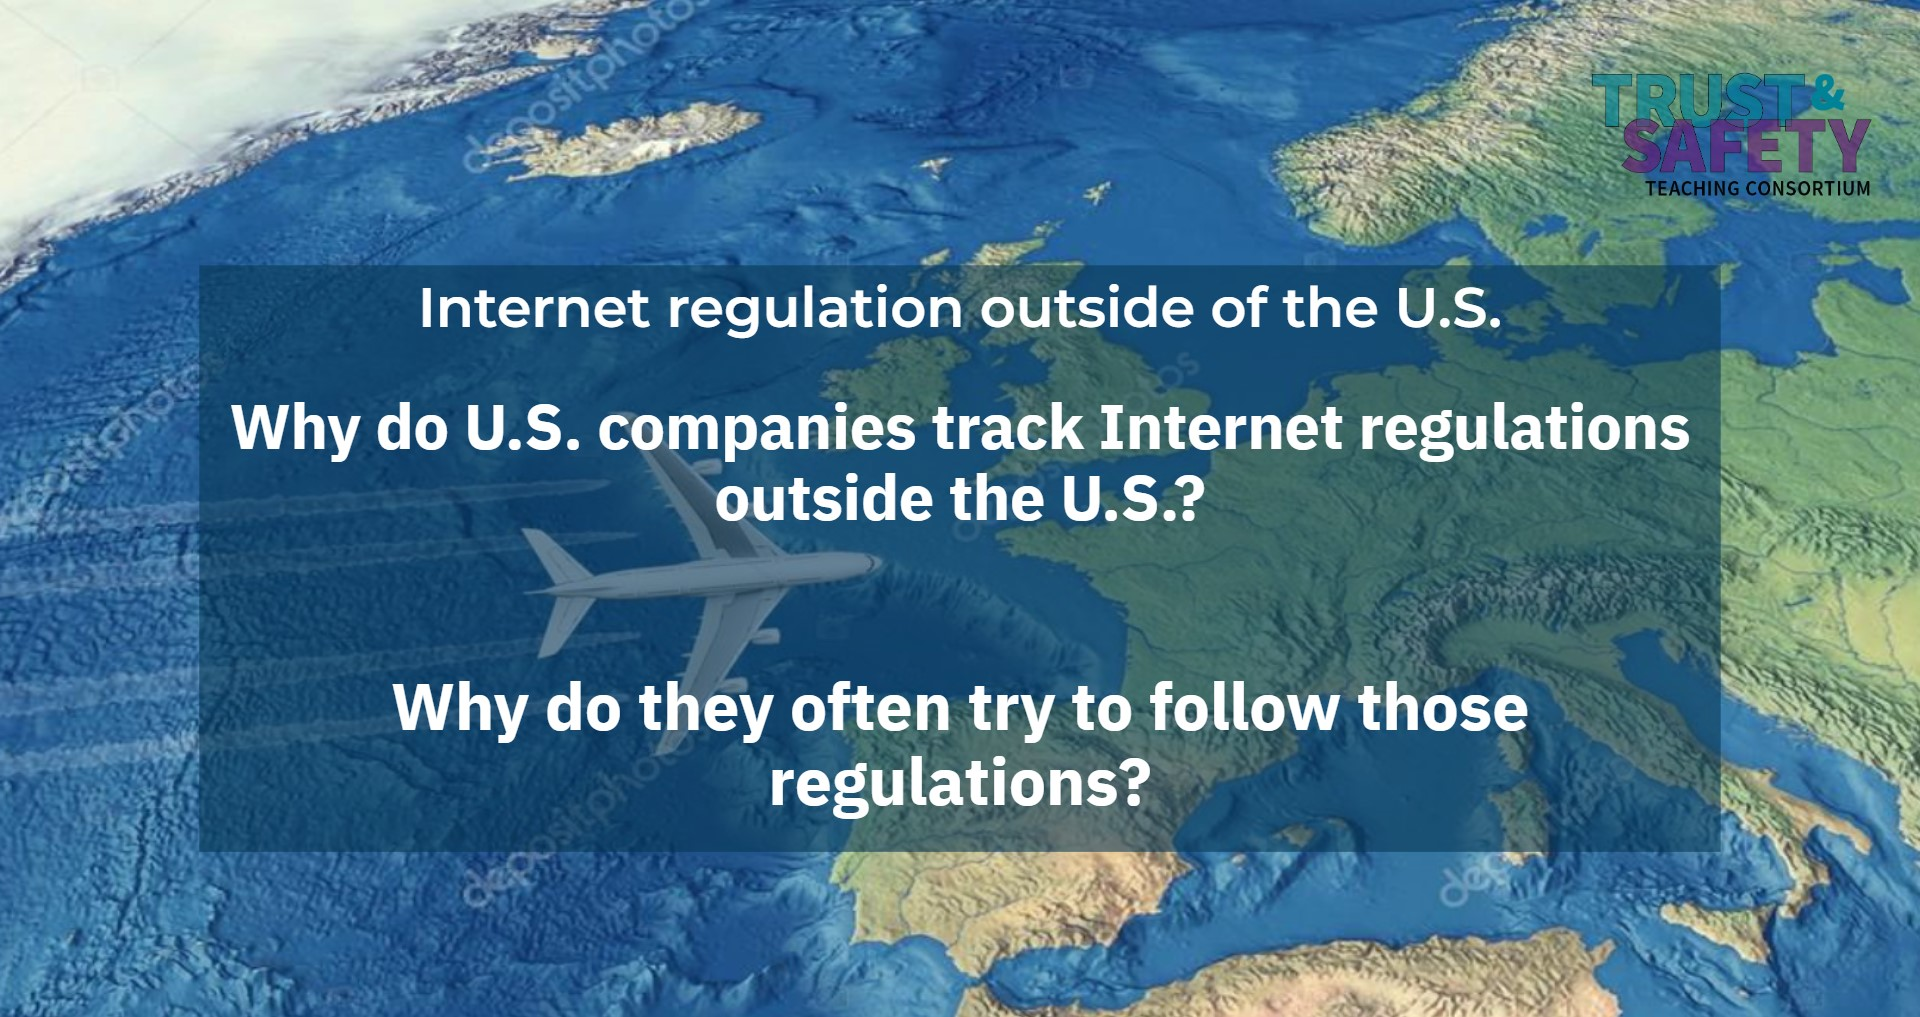
\includegraphics[width = \textwidth]{img/plane_picture.jpg}

\note[]{Ask students to give some reasons why US companies have to think about the laws outside of the U.S.}
\end{frame}


%%%%%%%%%%%%%%%%%%%%%%%%%%%%%%%%%%
%%%% slide 13 on google slides %%%%
%%%%%%%%%%%%%%%%%%%%%%%%%%%%%%%%%%
\begin{frame}{Some reasons why U.S. companies try to follow non-U.S. laws}
\begin{itemize}
    \item To make money. There are lucrative potential customers and users all over the world, particularly in rich countries. If you want to sell into Europe, you need to obey European laws.
    \item Companies may have legal entities in other jurisdictions for tax reasons, or licenses or permits to operate there. Those mean you need to follow the laws of those jurisdictions.
    \item Companies may have bank accounts, offices, factories, and employees in other countries. Some countries \emph{require} companies to have at least one employee on the ground in order to do business there. These are powerful levers that governments use get companies to obey their laws.
\end{itemize}

\note[]{India, for example, has a requirement to have an employee on the ground. \newline

Example of the Brussels Effect: All those cookie warnings you get come originally from European regulations. Note that you’ll see them even when you’re not in Europe or the other places where they’re now required. Showing them to everyone is easier than segmenting.} 

\end{frame}

\begin{frame}{Some reasons why U.S. companies try to follow non-U.S. laws}
%\footnotesize{
%\begin{itemize}
%    \item To make money. There are lucrative potential customers and users all over the world, particularly in rich countries. If you want to sell into Europe, you need to obey European laws.
%    \item Companies may have legal entities in other jurisdictions for tax reasons, or licenses or permits to operate there. Those mean you need to follow the laws of those jurisdictions.
%    \item Companies may have bank accounts, offices, factories, and employees in other countries. Some countries \emph{require} companies to have at least one employee on the ground in order to do business there. These are powerful levers that governments use get companies to obey their laws.
%\end{itemize}}

\large{\color{red!70}{\emph{Powerful jurisdictions like CA or the EU can make law for the entire world. They have enough clout that companies will try to comply with their laws, and other jurisdictions will use their laws as models for their own. Since it’s often easier for a platform to have one rule for all its users, practices required by the EU’s GDPR (for example) are applied to everyone. We call this “The Brussels Effect”.
}}}

\note[]{India, for example, has a requirement to have an employee on the ground. \newline

Example of the Brussels Effect: All those cookie warnings you get come originally from European regulations. Note that you’ll see them even when you’re not in Europe or the other places where they’re now required. Showing them to everyone is easier than segmenting.} 

\end{frame}


%%%%%%%%%%%%%%%%%%%%%%%%%%%%%%%%%%
%%%% slide 14 on google slides %%%%
%%%%%%%%%%%%%%%%%%%%%%%%%%%%%%%%%%
\begin{frame}{How companies make decisions about global internet speech laws - case study}

\footnotesize{
You’re the head of T\&S at a podcasting platform based in SF.  On Sunday night at 9:00 pm PT, you get an urgent note from Arvind, your company’s Grievance Officer based in Hyderabad - a position that India’s laws require. Arvind just received a letter from India’s tech regulator, MeitY, instructing you to immediately remove a podcast episode called “Modi in Gujarat: The Truth About the Riots”. The letter asserts that the episode is “defamatory and a threat to public order,” which are grounds for MeitY to demand content be removed under India’s intermediary liability laws. You have 8m users in India and an engineering office in Hyderabad with 10 employees.\newline

MeitY’s letter also contains an official request for the name, address, IP address, and login history of the podcast host, who uses a pseudonym on your platform. Under Indian intermediary laws, you have \textbf{36 hours} to remove the episode and \textbf{72 hours} to return the information to MeitY. The official from MeitY has asked your Grievance Officer to come in to discuss the matter Tuesday morning IST.\newline}

\textbf{What happens next?}

\end{frame}


%%%%%%%%%%%%%%%%%%%%%%%%%%%%%%%%%%
%%%% slide 15 on google slides %%%%
%%%%%%%%%%%%%%%%%%%%%%%%%%%%%%%%%%
\begin{frame}{Chronology}

Letter received Sunday 9 PM / + 36 hours is \textbf{Tuesday 10 AM} / + 72 hours is \textbf{Weds 10 PM}\newline

India Standard Time is 12.5 hours ahead of PT

\begin{center}
    \rule{8cm}{0.4pt}    
\end{center}

\small{
\begin{itemize}
    \item Who in your company should you add to the new chat channel for this issue?
    \item Who should you consult outside the company?
    \item What additional information would you like to have?
    \item What can you do to try to buy more time?
    \item Should Arvind meet with MeitY at its office on Tuesday morning IST? What can we do to keep him safe?
    \item How to protect the 10 engineers in the Hyderabad office? How to talk about what’s going on?
\end{itemize}
}

\note[]{When reviewing the list of people who should be involved, ask students to identify what the priorities of those individuals are.  What is the head comms person thinking most about? The COO? The head of gov’t relations? Your outside counsel? Arvind? Arvind’s family?
}
\end{frame}

%%%%%%%%%%%%%%%%%%%%%%%%%%%%%%%%%%
%%%% slide 16 on google slides %%%%
%%%%%%%%%%%%%%%%%%%%%%%%%%%%%%%%%%
\begin{frame}{}

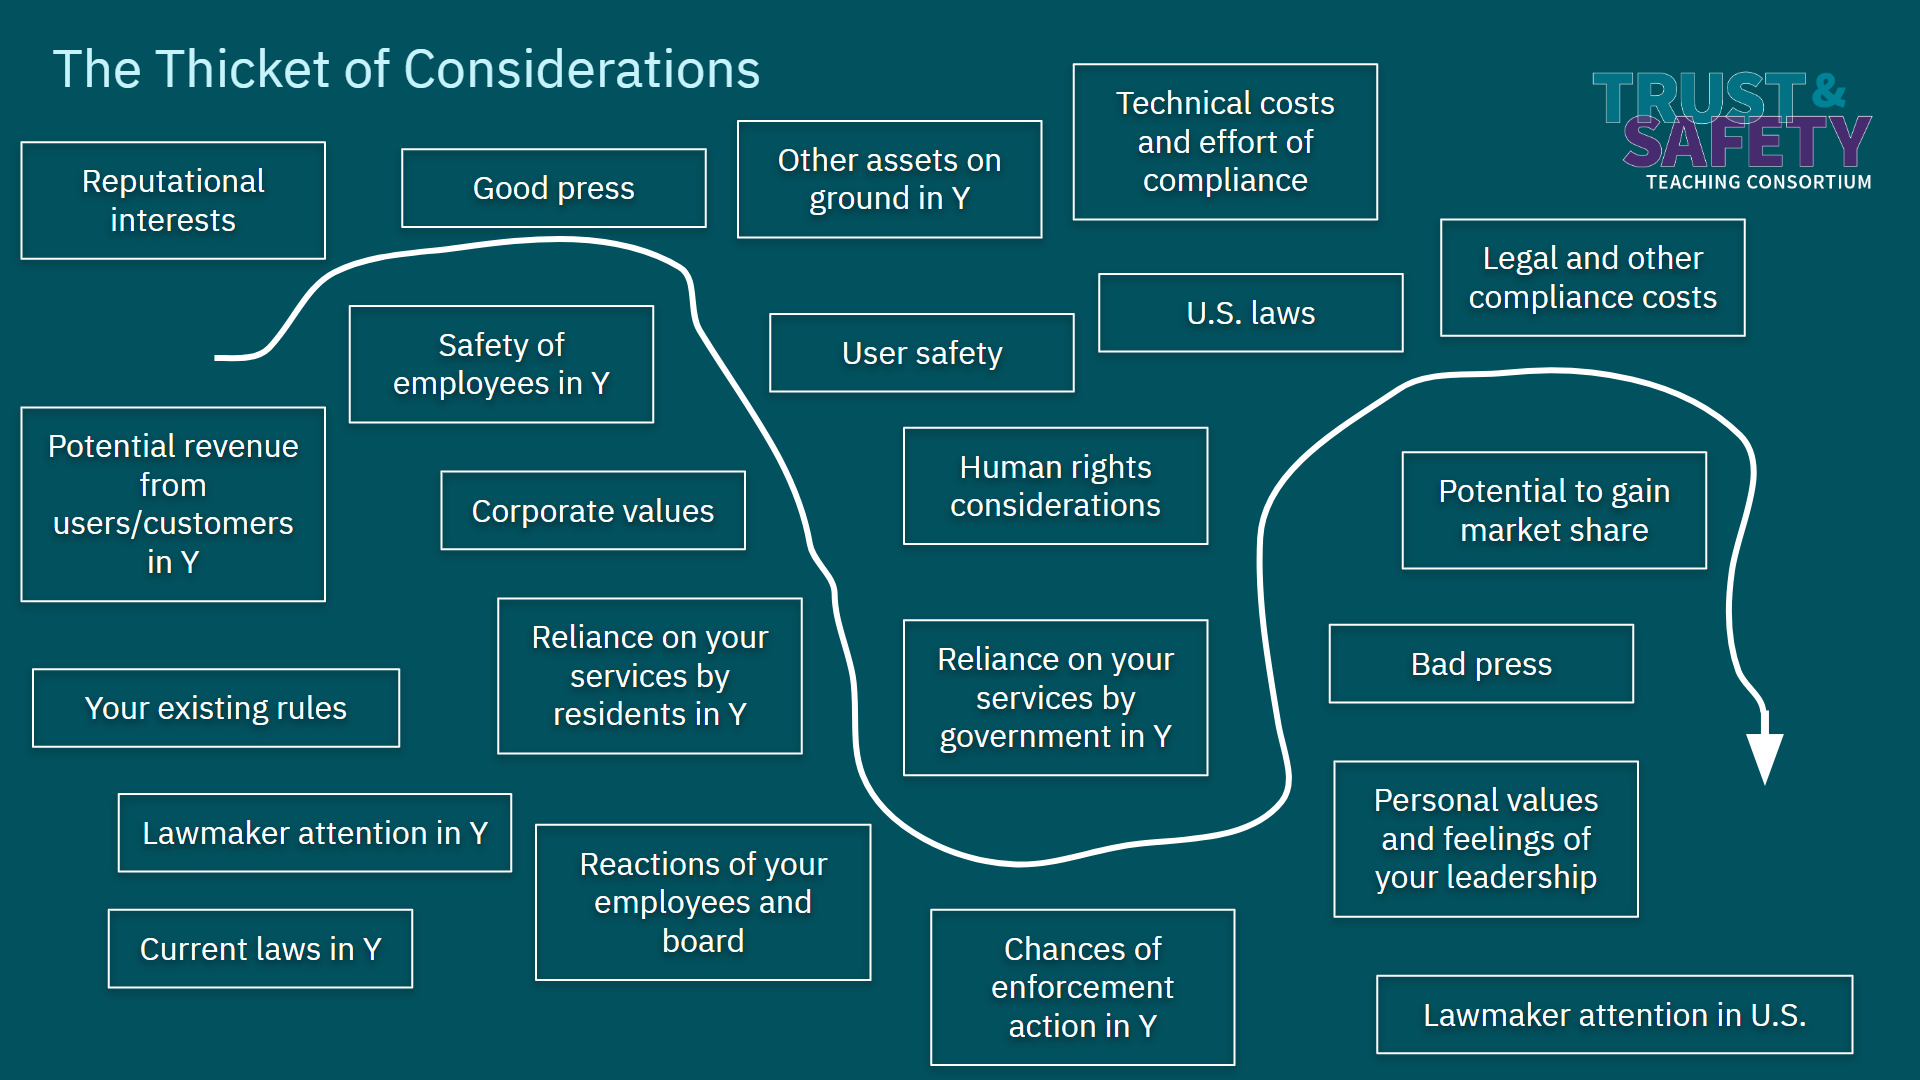
\includegraphics[width = \textwidth]{img/slide_16_picture.png}

\note[]{

\footnotesize{
Examples of decisions: 
\begin{enumerate}
    \item Do we take down content that’s suddenly high profile and controversial in country Y?
    \item What do we do about a new intermediary liability law in country Y?
\end{enumerate}


At big established companies, there are likely processes and playbooks for making these decisions. A lot of people will help make the decision. At smaller companies, the decisionmaking will feel more ad hoc and it might be a single person making the call. \newline \newline But the general set of considerations is the same. The tensions among “free speech”, “user safety”, “making money”, “complying with all laws wherever you do business” are not resolvable. The best you can do is try to manage the tensions over time, to thread a careful path and focus more on good process.}
}

\end{frame}

%\backpage

\end{document}